 

\section*{Aufgabe 1: \emph{Zwei Populationen}}


\begin{figure}
	\centering
	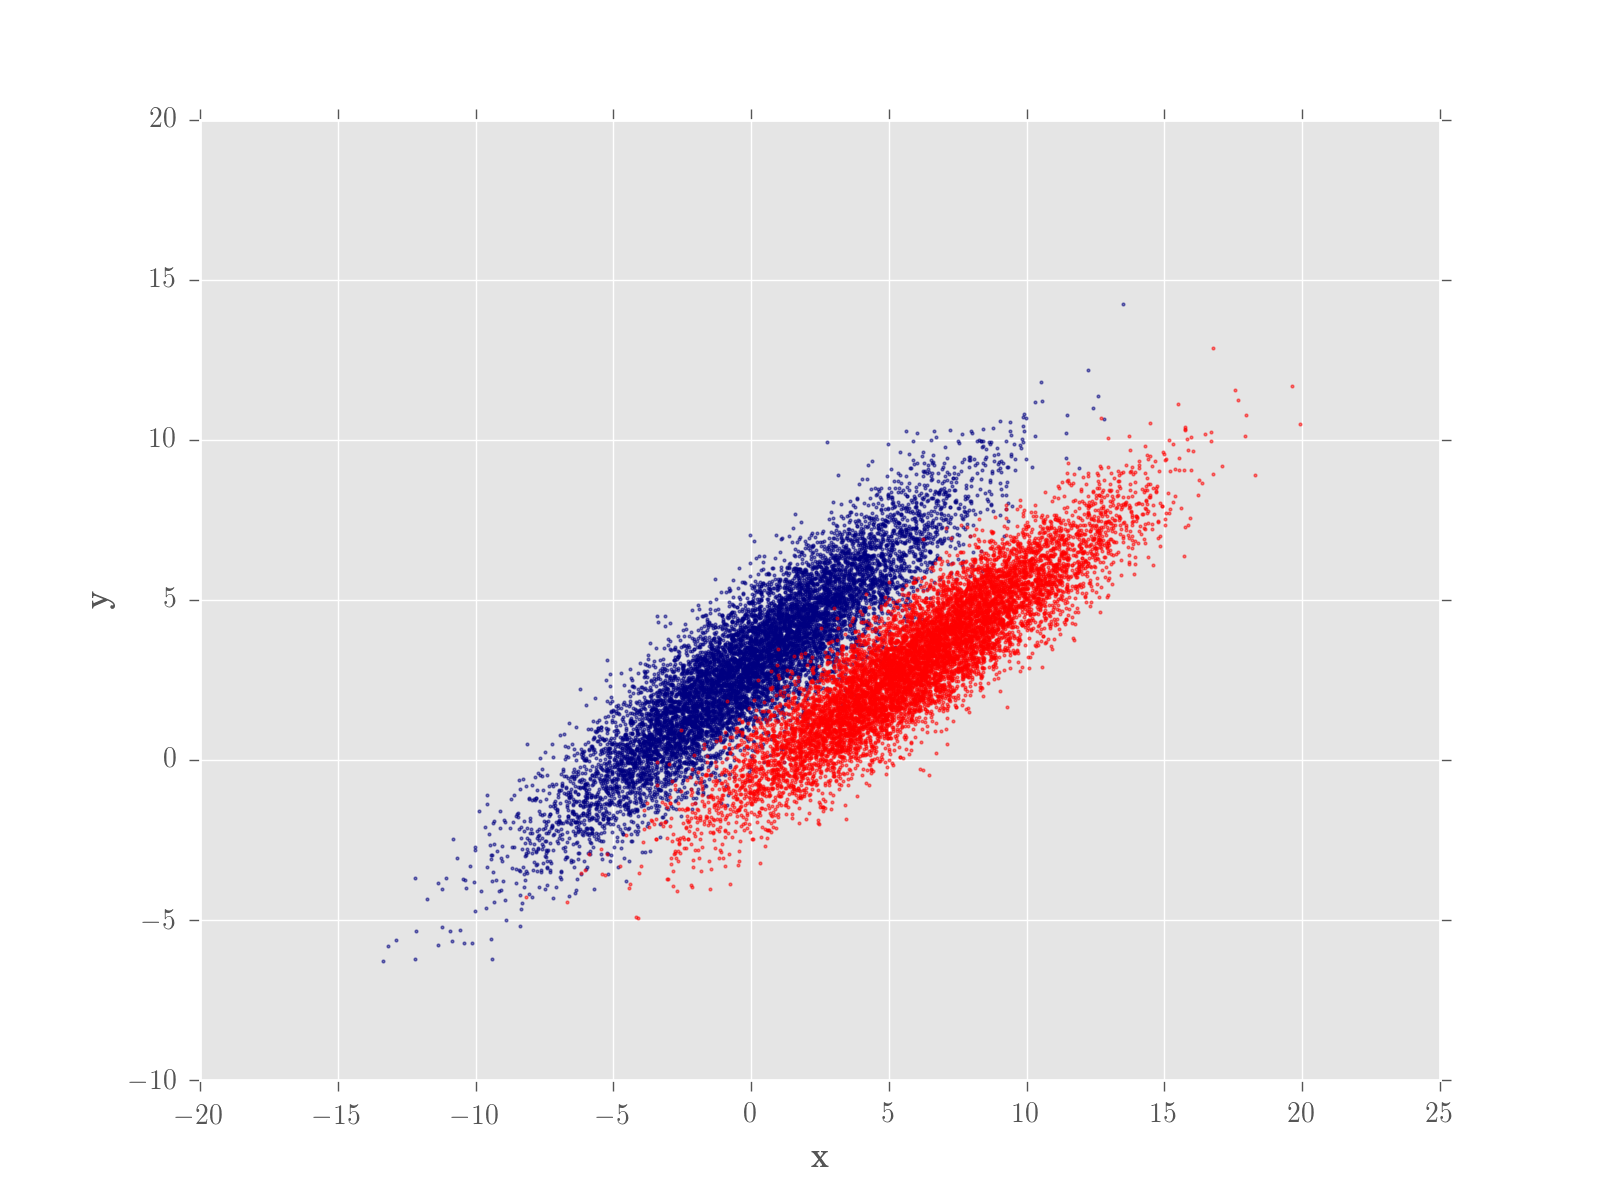
\includegraphics[width=0.7\textwidth]{1b.png}
	\caption{Zweidimensionaler Scatterplot der Populationen.}
\end{figure}
\begin{itemize}
\item[c)]
Die Stichprobenmittelwerte sind $x_{\text{mean}} = 6.026$ und $y_{\text{mean}} = 3.125$,
Die Varianzen sind $var_x = 12.225$ und $var_y = 5.365$.
Die Kovarianz ist $cov_xy = 7.321$ und der Korellationskoeffizient $\rho_{xy} = 0.904$
\end{itemize}


\section*{Aufgabe 2: \emph{Trennende Geraden}}

\begin{figure}
	\centering
	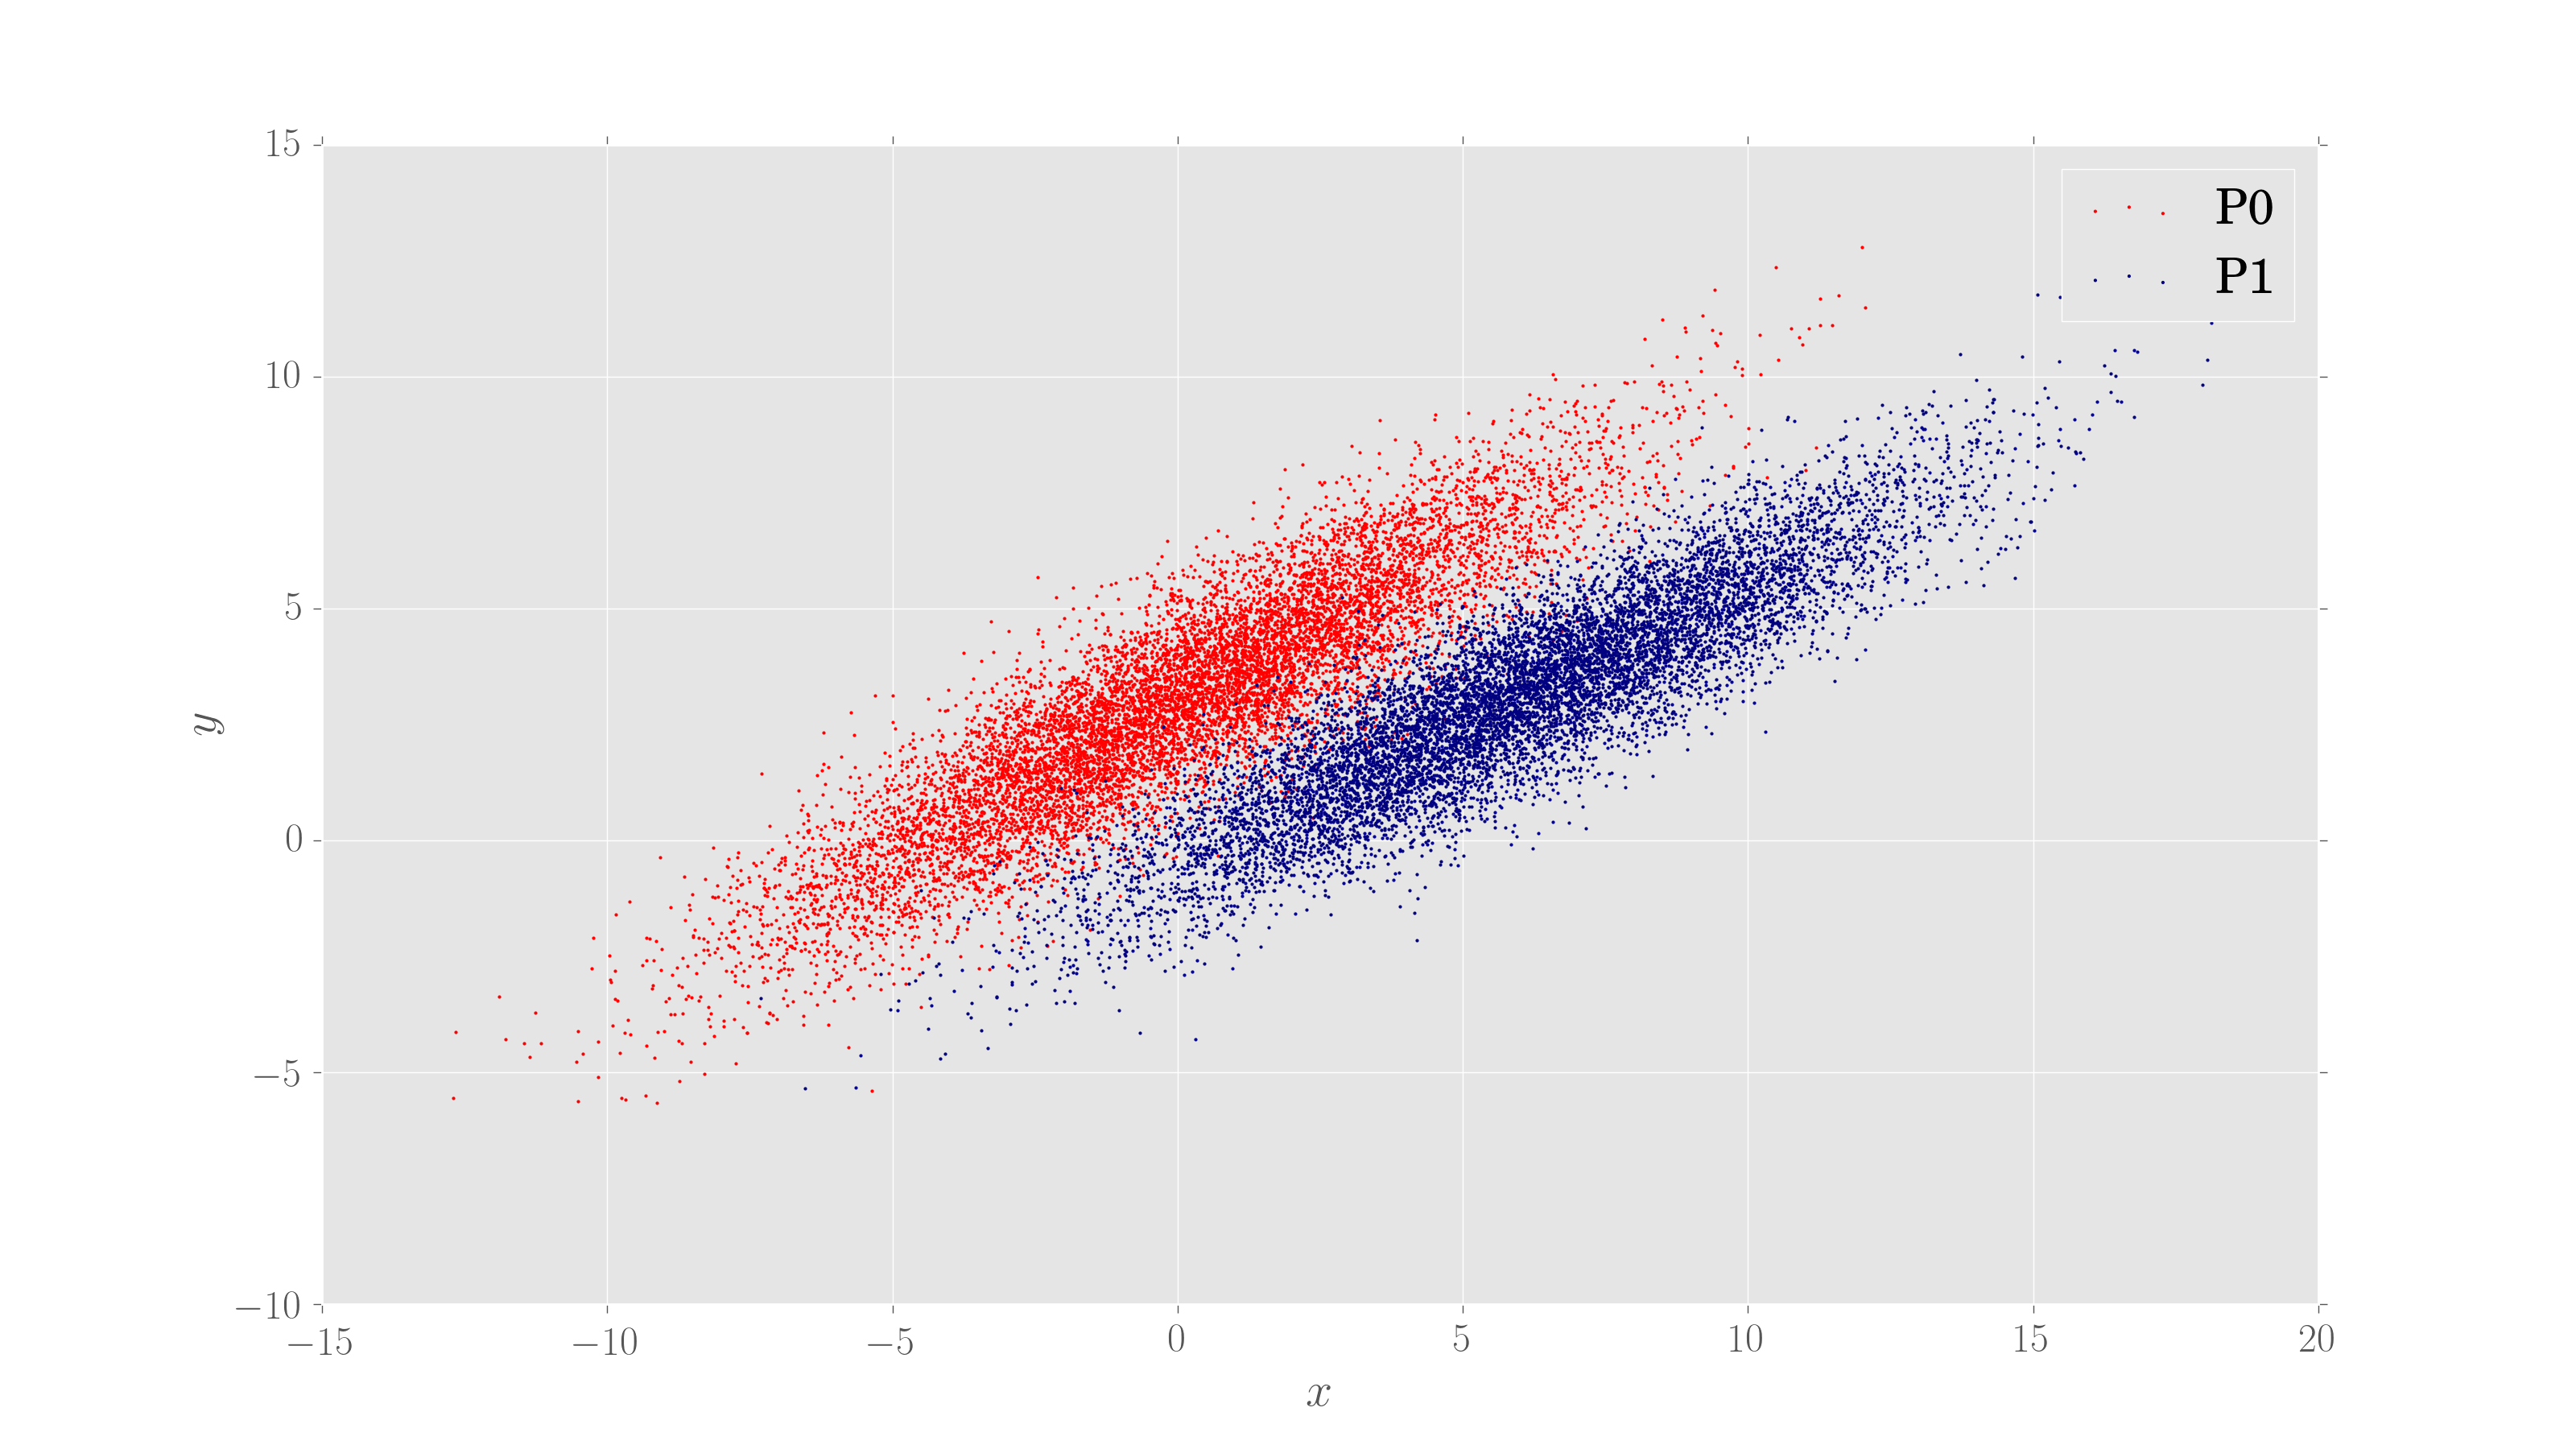
\includegraphics[width=0.7\textwidth]{scatter_P0_P1.png}
	\caption{Zweidimensionaler Scatterplot der Populationen.}
\end{figure}
\begin{figure}
	\centering
	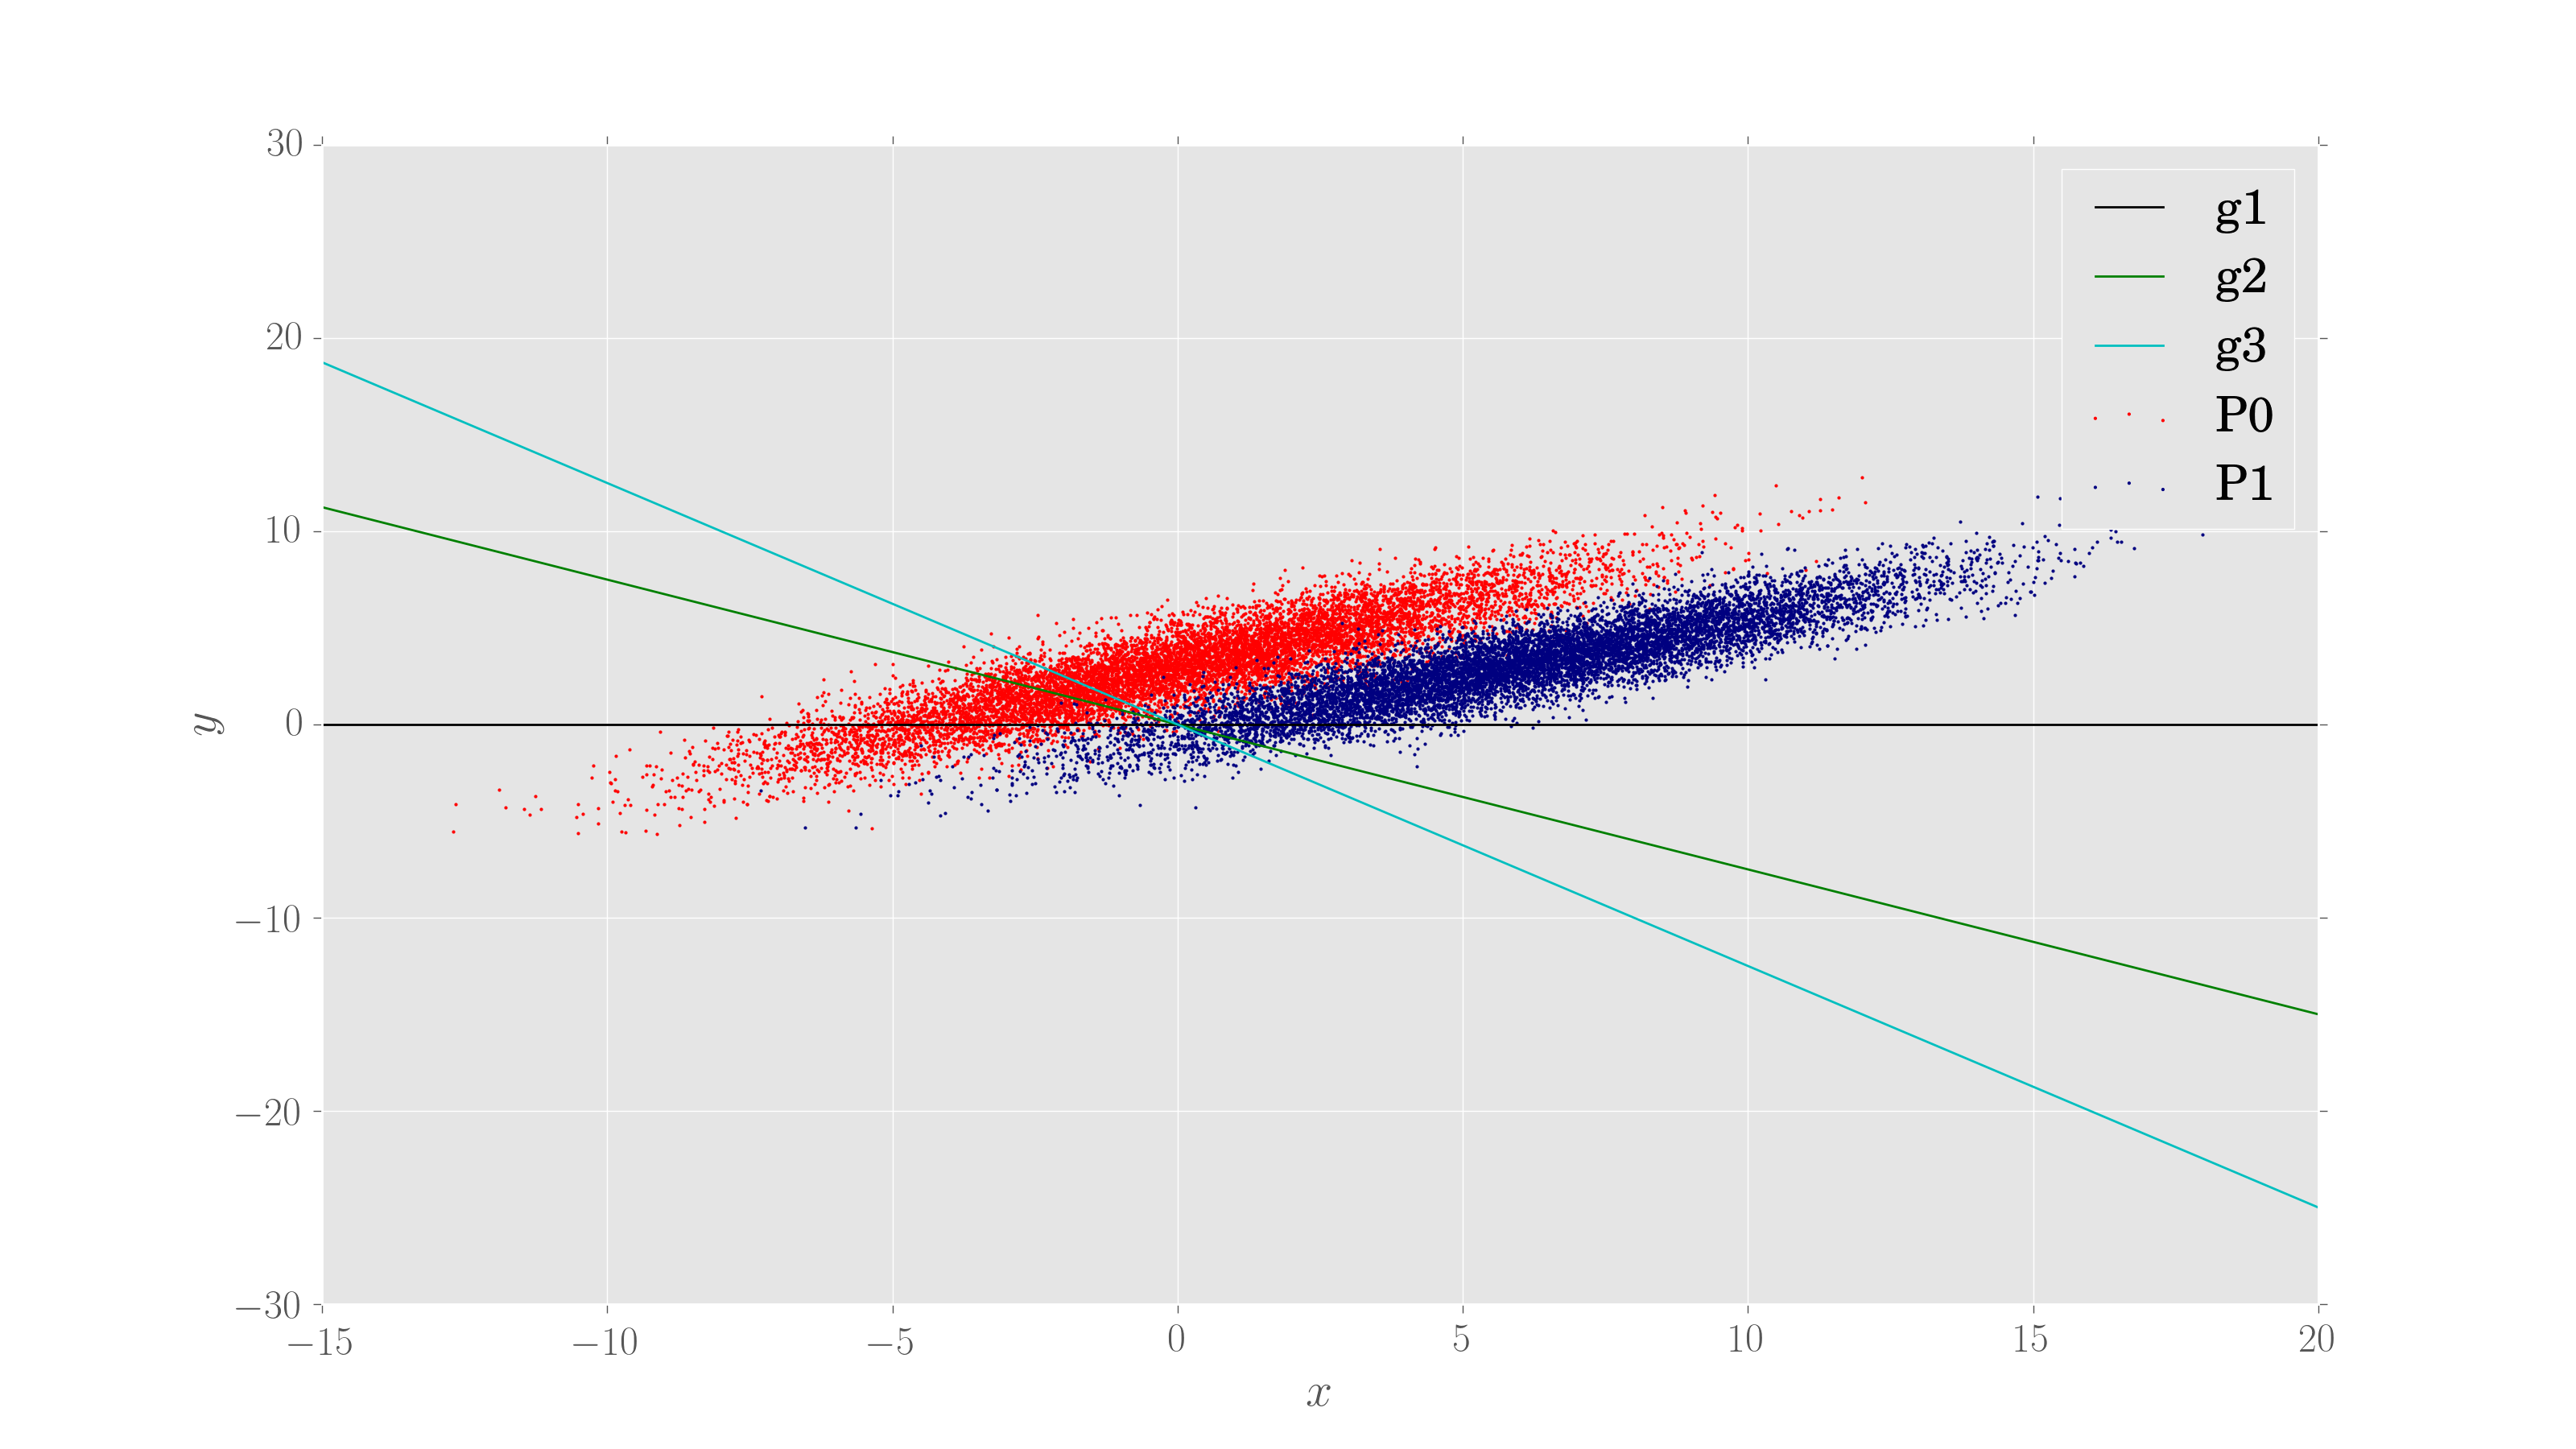
\includegraphics[width=0.7\textwidth]{scatter_with_lines.png}
	\caption{Zweidimensionaler Scatterplot der Populationen mit eingezeichneten Projektionsgeraden.}
\end{figure}
\begin{figure}
	\centering
	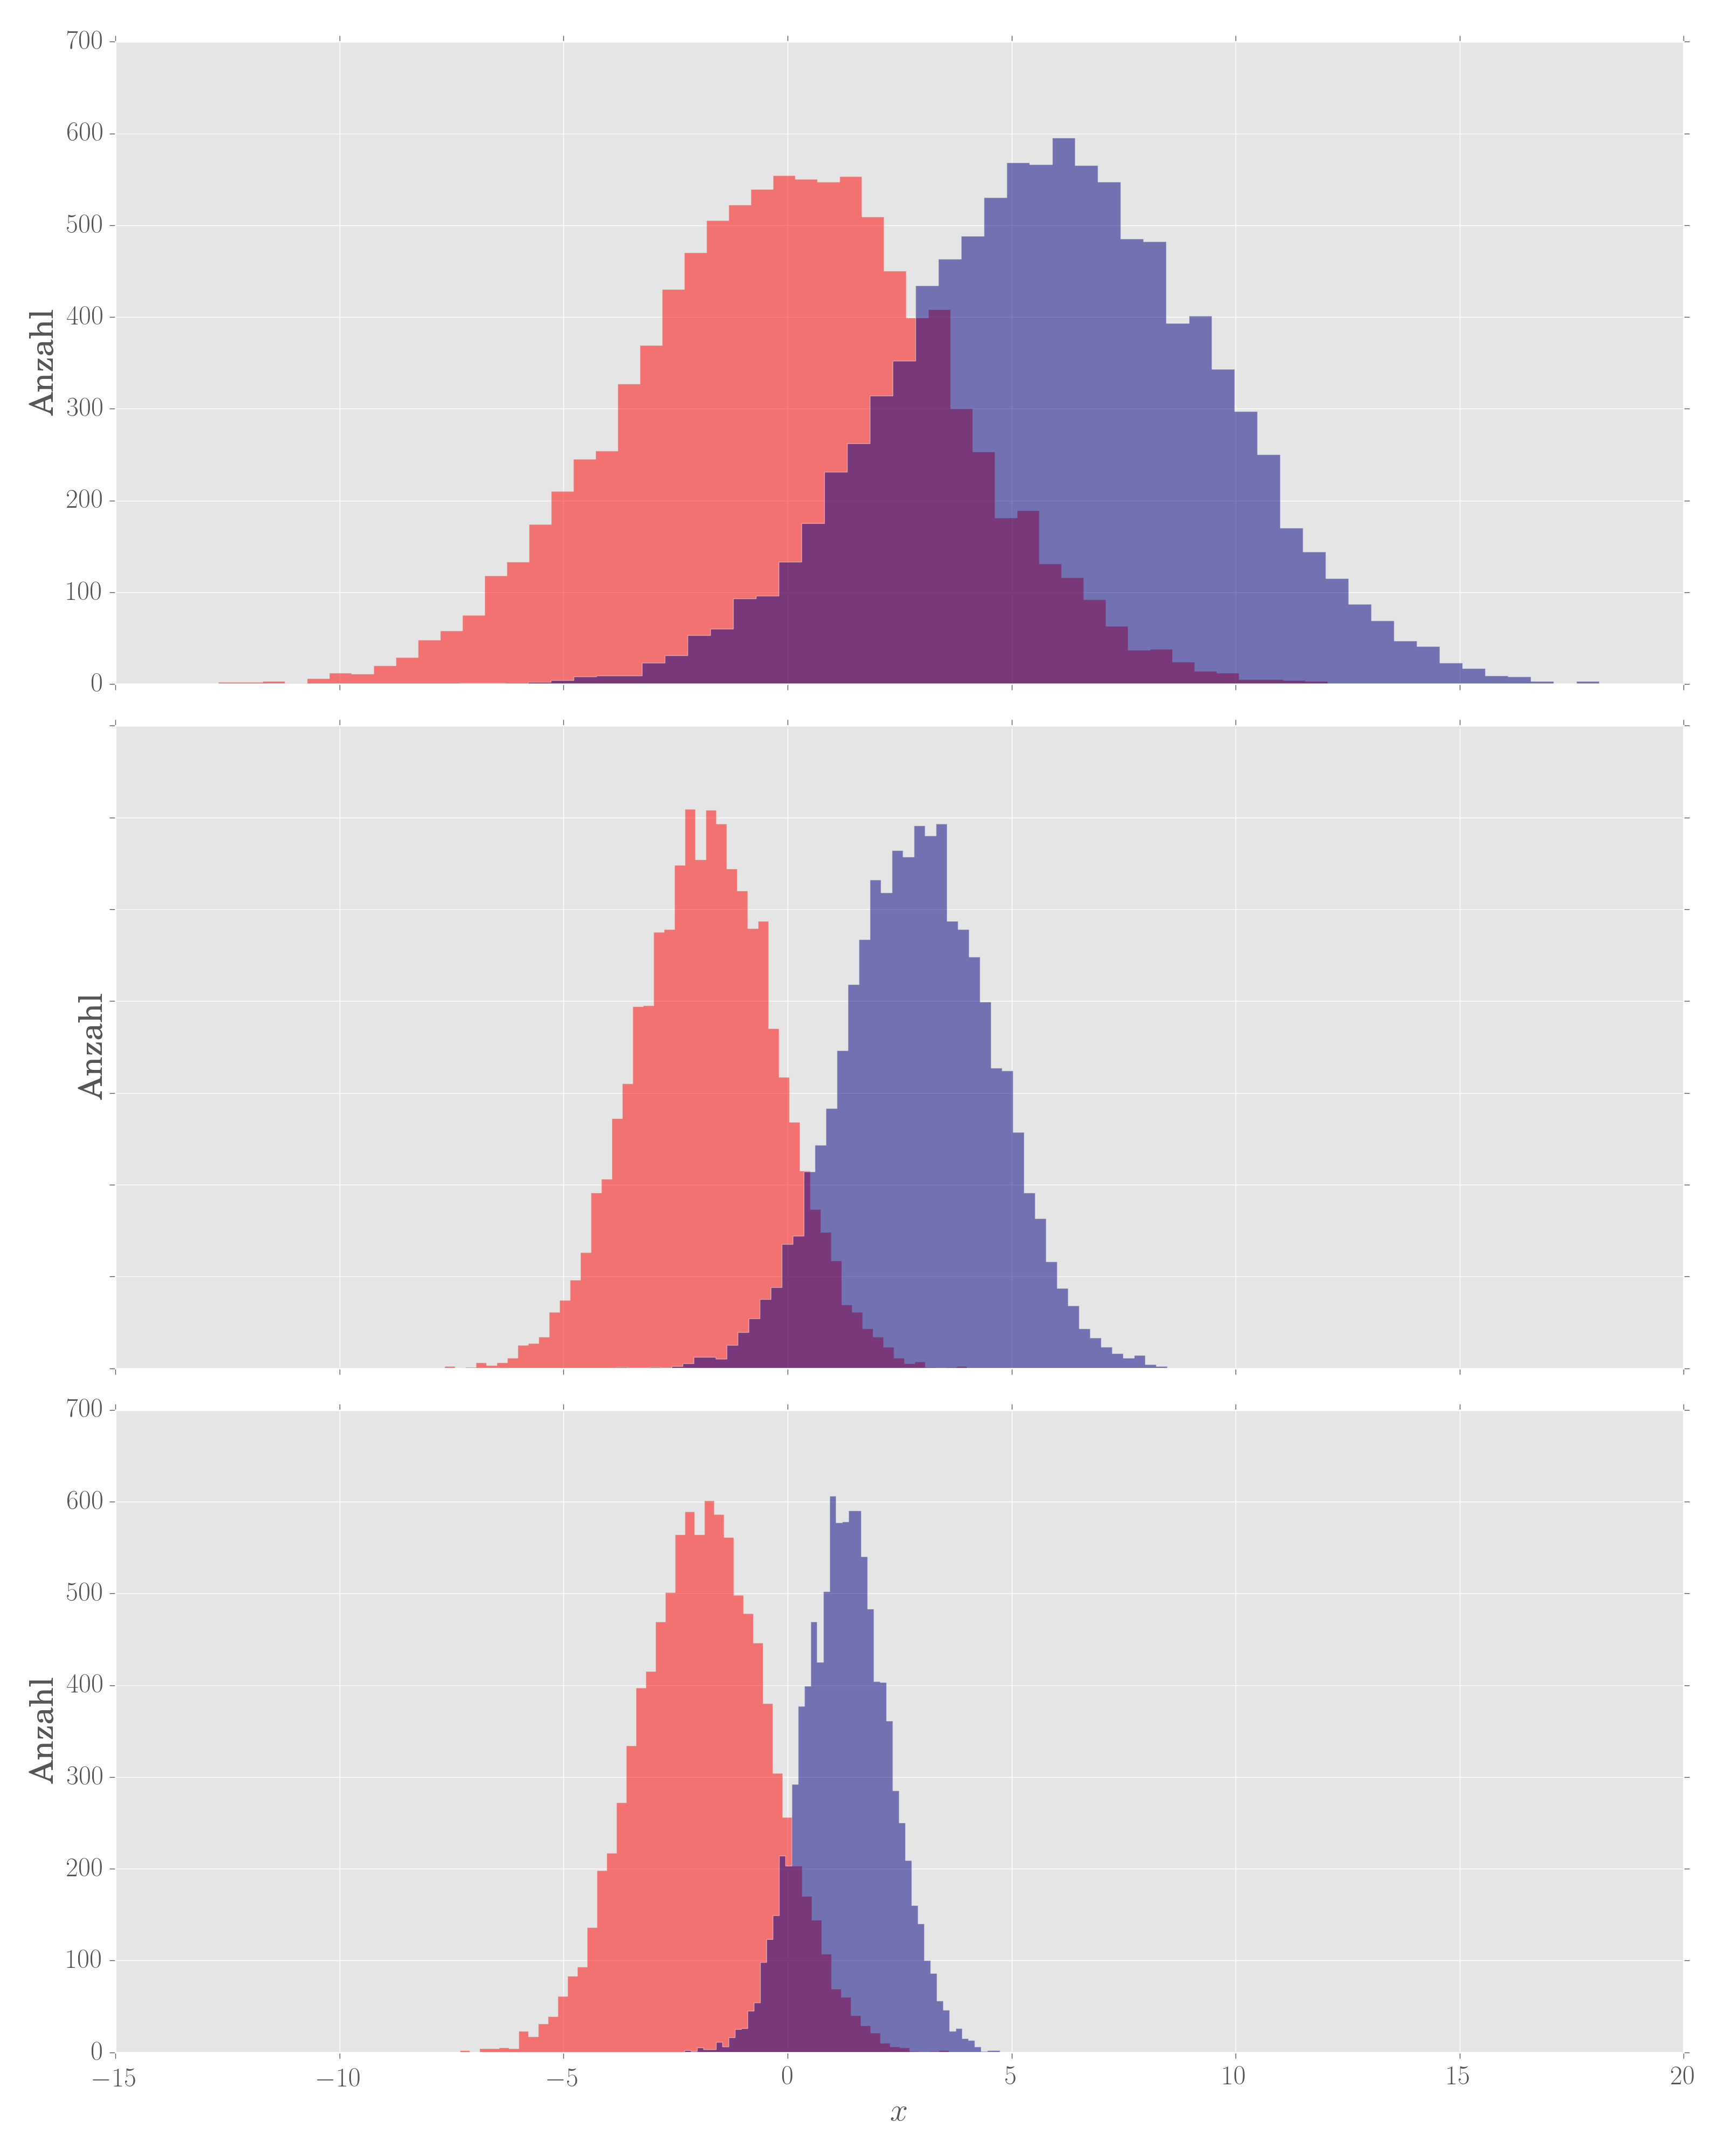
\includegraphics[width=0.7\textwidth]{hists_proj.png}
	\caption{Projektion der Populationen auf die Geraden $g_1$,$g_2$ und $g_3$}
\end{figure}

\begin{figure}
	\centering
	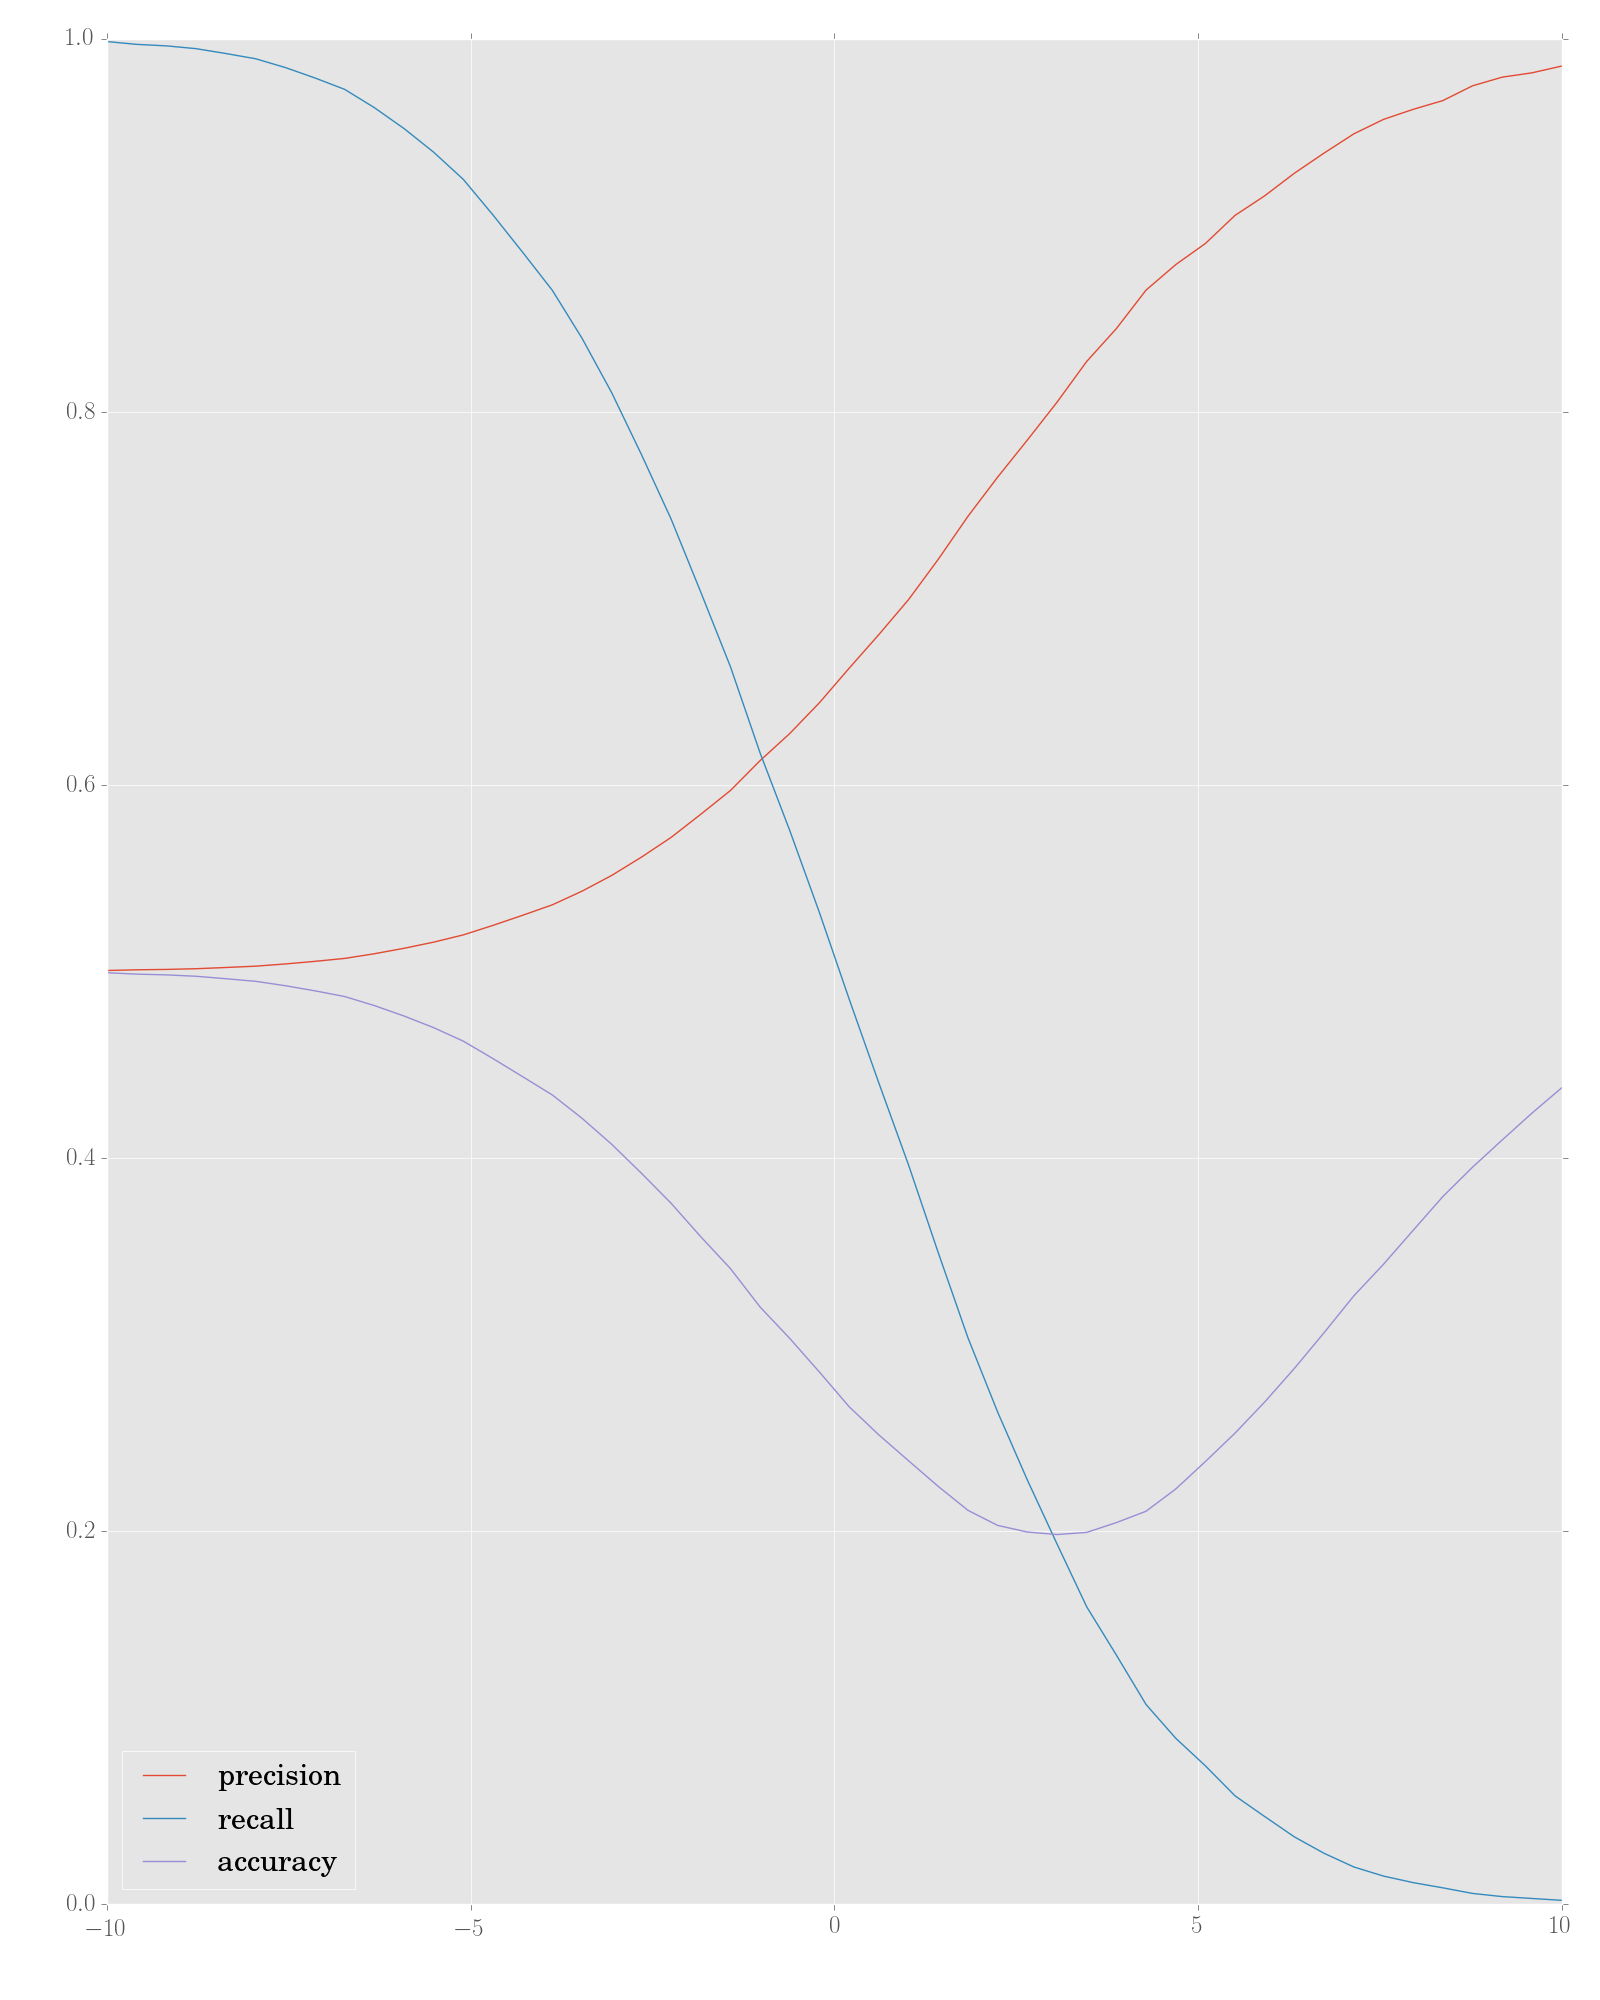
\includegraphics[width=0.7\textwidth]{performace_g1.png}
	\caption{Reinheit (precision), Effizienz (accuracy) und Sensitivität (recall) für die Gerade $g_1$}
\end{figure}
\begin{figure}
	\centering
	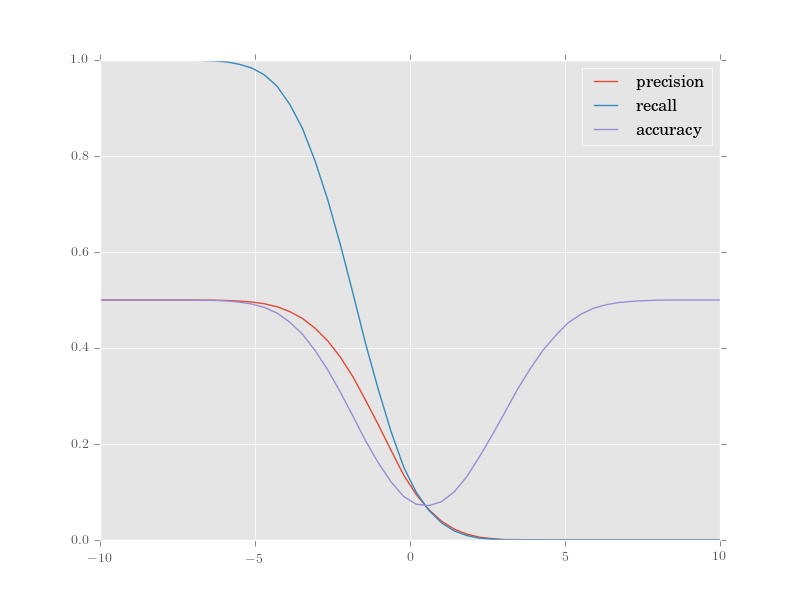
\includegraphics[width=0.7\textwidth]{performace_g2.png}
	\caption{Reinheit (precision), Effizienz (accuracy) und Sensitivität (recall) für die Gerade $g_2$}
\end{figure}

\begin{figure}
	\centering
	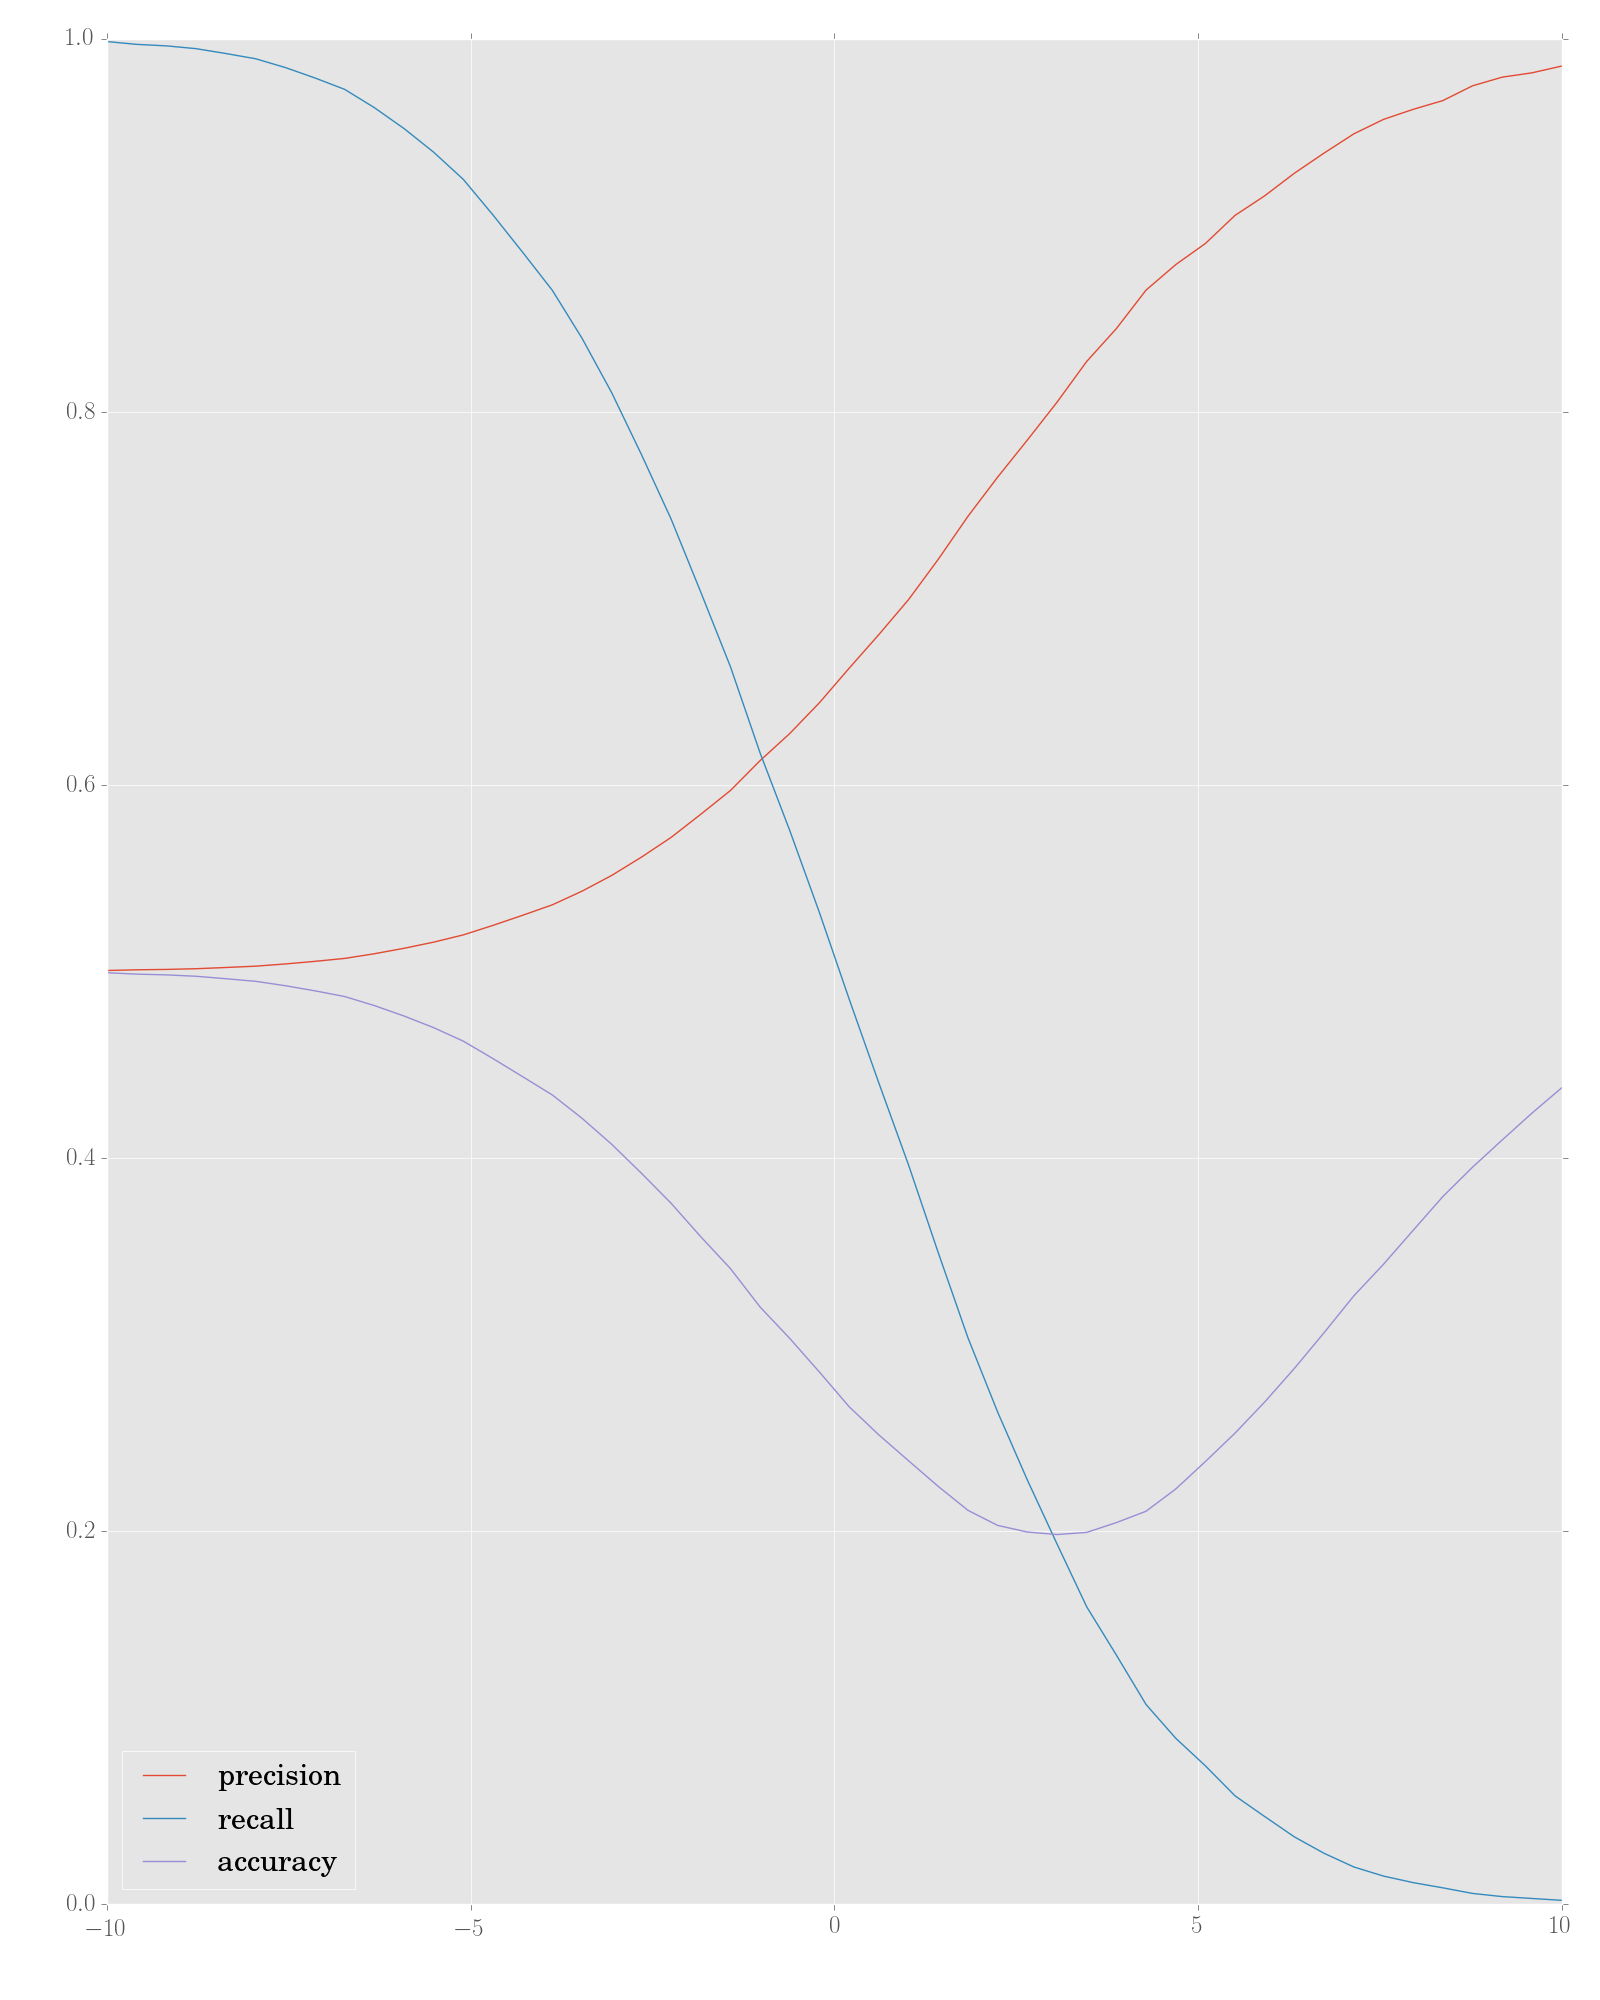
\includegraphics[width=0.7\textwidth]{performace_g1.png}
	\caption{Reinheit (precision), Effizienz (accuracy) und Sensitivität (recall) für die Gerade $g_3$}
\end{figure}



\section*{Aufgabe 3: \emph{Fisher--Diskrimanante: Per Hand}}
\textbf{a) Mittelwerte und Streumatrizen zu P0 und P1} \\
Population $P_0$:
\[
\vec{p}_1 =
\left(
\begin {array} {c}

2 \\

2 \\

1 \\

\end {array}
\right)
, \qquad
\vec{p}_2 =
\left(
\begin {array} {c}

2 \\

3 \\

2 \\

\end {array}
\right)
, \qquad
\vec{p}_3 =
\left(
\begin {array} {c}

1 \\

2 \\

0 \\

\end {array}
\right)
, \qquad
\vec{p}_4 =
\left(
\begin {array} {c}

3 \\

2 \\

0 \\

\end {array}
\right)
, \qquad
\vec{p}_5 =
\left(
\begin {array} {c}

2 \\

1 \\

2 \\

\end {array}
\right)
\]
\\
Population $P_1$:
\[
\vec{q}_1 =
\left(
\begin {array} {c}

2,5 \\

2,5 \\

0 \\

\end {array}
\right)
, \qquad
\vec{q}_2 =
\left(
\begin {array} {c}

2,5 \\

1,5 \\

0 \\

\end {array}
\right)
, \qquad
\vec{q}_3 =
\left(
\begin {array} {c}

4 \\

2 \\

0 \\

\end {array}
\right)
, \qquad
\vec{q}_4 =
\left(
\begin {array} {c}

5,5 \\

2,5 \\

0 \\

\end {array}
\right)
, \qquad
\vec{q}_5 =
\left(
\begin {array} {c}

5,5 \\

1,5 \\

0 \\

\end {array}
\right)
\]
Bestimmung der Mittelwerte $\mu_i$:
\[
\vec{\mu}_0 = \frac{1}{N_0} \sum{p_i} = \frac{1}{5}
\left(
\begin {array} {c}
2 + 2 + 1 + 3 + 2 \\
2 + 3 + 2 + 2 + 1 \\
1 + 2 + 0 + 0 + 2 \\
\end{array}
\right)
= \frac{1}{5}
\left(
\begin {array} {c}
10 \\
10 \\
5 \\
\end {array}
\right)
=
\left(
\begin {array} {c}
2 \\
2 \\
1 \\
\end {array}
\right)
\]
\[
\vec{\mu}_1 = \frac{1}{N_1} \sum{q_i} = \frac{1}{5}
\left(
\begin {array} {c}
2,5 + 2,5 + 4 + 5,5 + 5,5 \\
2,5 + 1,5 + 2 + 2,5 + 1,5 \\
0 + 0 + 0 + 0 + 0 \\
\end{array}
\right)
= \frac{1}{5}
\left(
\begin {array} {c}
20 \\
10 \\
0 \\
\end {array}
\right)
=
\left(
\begin {array} {c}
4 \\
2 \\
0 \\
\end {array}
\right)
\]
Streuung der Klasse $S_j = \sum{(\vec{x}_i - \vec{\mu}_i)(\vec{x}_i - \vec{\mu}_i)^T}$: \\
Streumatrix $S_0$:
\[ 
\left(
\begin {array} {c}
2 - 2 \\
2 - 2 \\
1 - 1 \\
\end {array}
\right)
\left(
\begin {array} {c}
2 - 2 \qquad 2 - 2 \qquad 1 - 1 
\end {array}
\right) 
+
\left(
\begin {array} {c}
2 - 2 \\
3 - 2 \\
2 - 1 \\
\end {array}
\right)
\left(
\begin {array} {c}
2 - 2 \qquad 3 - 2 \qquad 2 - 1 
\end {array}
\right)
+ \qquad \cdots \\ 
\]
\[
= 
\left(
\begin {array} {c}
0 \\
0 \\
0 \\
\end {array}
\right)
\left(
\begin {array} {c}
0 \qquad 0 \qquad 0 
\end {array}
\right) 
+
\left(
\begin {array} {c}
0 \\
1 \\
1 \\
\end {array}
\right)
\left(
\begin {array} {c}
0 \qquad 1 \qquad 1 
\end {array}
\right)
+ \qquad \cdots
\]
\[
= 
\left(
\begin {array} {c}
0 \qquad 0 \qquad 0 \\
0 \qquad 0 \qquad 0  \\
0 \qquad 0 \qquad 0  \\
\end {array}
\right)
+
\left(
\begin {array} {c}
0 \qquad 0 \qquad 0  \\
0 \qquad 1 \qquad 1  \\
0 \qquad 1 \qquad 1  \\
\end {array}
\right)
+
\left(
\begin {array} {c}
1 \qquad 0 \qquad 1  \\
0 \qquad 0 \qquad 0  \\
1 \qquad 0 \qquad 1  \\
\end {array}
\right)
+ \qquad \cdots
\]
\[
S_0 =
\left(
\begin {array} {c}
2 \qquad 0 \qquad 0  \\
0 \qquad 2 \qquad 0  \\
0 \qquad 0 \qquad 4  \\
\end {array}
\right)
\]
Streumatrix $S_1$: 
\[
\left(
\begin {array} {c}
2,5 - 4 \\
2,5 - 2 \\
0 - 0 \\
\end {array}
\right)
\left(
\begin {array} {c}
2,5 - 4 \qquad 2,5 - 2 \qquad 0 - 0 
\end {array}
\right)
\]
\[ 
+
\left(
\begin {array} {c}
2,5 - 4 \\
1,5 - 2 \\
0 - 0 \\
\end {array}
\right)
\left(
\begin {array} {c}
2,5 - 4 \qquad 1,5 - 2 \qquad 0 - 0 
\end {array}
\right)
+ \qquad \cdots \\ 
\]
\[
= 
\left(
\begin {array} {c}
-1,5 \\
0,5 \\
0 \\
\end {array}
\right)
\left(
\begin {array} {c}
-1,5 \qquad 0,5 \qquad 0 
\end {array}
\right)
+
\left(
\begin {array} {c}
-1,5 \\
-0,5 \\
0 \\
\end {array}
\right)
\left(
\begin {array} {c}
-1,5 \qquad -0,5 \qquad 0 
\end {array}
\right) 
+ \qquad \cdots
\]
\[
= 
\left(
\begin {array} {c}
2,25 \qquad -0,75 \qquad 0 \\
-0,75 \qquad 0,25 \qquad 0  \\
0 \qquad 0 \qquad 0  \\
\end {array}
\right)
+
\left(
\begin {array} {c}
2,25 \qquad 0,75 \qquad 0 \\
0,75 \qquad 0,25 \qquad 0  \\
0 \qquad 0 \qquad 0  \\
\end {array}
\right)
+
\left(
\begin {array} {c}
0 \qquad 0 \qquad 0  \\
0 \qquad 0 \qquad 0  \\
0 \qquad 0 \qquad 0  \\
\end {array}
\right)
+ \qquad \cdots
\]
\[
S_1 =
\left(
\begin {array} {c}
9 \qquad 0 \qquad 0  \\
0 \qquad 1 \qquad 0  \\
0 \qquad 0 \qquad 0  \\
\end {array}
\right)
\]
Fuer die Streuung innerhalb der Klassen $S_W$ ergibt sich:
\[
S_W = \sum{S_i} = 
\left(
\begin {array} {c}
2 \qquad 0 \qquad 0  \\
0 \qquad 2 \qquad 0  \\
0 \qquad 0 \qquad 4  \\
\end {array}
\right)
+
\left(
\begin {array} {c}
9 \qquad 0 \qquad 0  \\
0 \qquad 1 \qquad 0  \\
0 \qquad 0 \qquad 0  \\
\end {array}
\right)
=
\left(
\begin {array} {c}
11 \qquad 0 \qquad 0  \\
0 \qquad 3 \qquad 0  \\
0 \qquad 0 \qquad 4  \\
\end {array}
\right)
\]
Die Streuung zwischen den Klassen $S_B$ wird ueber die Mittelwerte $\mu_i$ bestimmt.
\[
S_B = (\vec{\mu}_0 - \vec{\mu}_1)(\vec{\mu}_0 - \vec{\mu}_1)^T = 
\left(
\begin {array} {c}
2 - 4 \\
2 - 2 \\
1 - 0 \\
\end {array}
\right)
\left(
\begin {array} {c}
2 - 4 \qquad 2 - 2 \qquad 1 - 0 \\
\end {array}
\right)
=
\left(
\begin {array} {c}
4 \qquad 0 \qquad -2  \\
0 \qquad 0 \qquad 0  \\
-2 \qquad 0 \qquad 1  \\
\end {array}
\right)
\]
\textbf{b) Eigenwerte und Eigenvektoren zu $S_W^{-1}S_B$} \\
Die inverse Matrix zu $S_W$ ist aufgrund ihrer Diagonalform leicht zu bestimmen. 
Dazu wird das Inverse der Elemente $a_{ii}$ bestimmt. Fuer $S_W^{-1}$ ergeben sich die Werte
$a_{11} = \frac{1}{11}$, $a_{22} = \frac{1}{3}$ und $a_{33} = \frac{1}{4}$.
Anschliessend bestimmen wir das Produkt dieser Matrix mit der $S_B$ Matrix:
\[
S_W^{-1}S_B =
\left(
\begin {array} {c}
\frac{1}{11} \qquad 0 \qquad 0  \\
0 \qquad \frac{1}{3} \qquad 0  \\
0 \qquad 0 \qquad \frac{1}{4}  \\
\end {array}
\right)
\left(
\begin {array} {c}
4 \qquad 0 \qquad -2  \\
0 \qquad 0 \qquad 0  \\
-2 \qquad 0 \qquad 1  \\
\end {array}
\right)
=
\left(
\begin {array} {c}
\frac{4}{11} \qquad 0 \qquad \frac{-2}{11}  \\
0 \qquad 0 \qquad 0  \\
\frac{-1}{2} \qquad 0 \qquad \frac{1}{4}  \\
\end {array}
\right)
\]
Um die Eigenwerte zu bestimmen, betrachten wir das Eigenwertproblem $(A - \lambda E) \vec{x} = 0$.
Ueber das charakteristische Polynom ermitteln wir dann die 3 Eigenwerte. Eingesetzt in
das Eigenwertproblem werden schliesslich die Eigenvektoren bestimmt.
\[
\left(
\left(
\begin {array} {c}
\frac{4}{11} \qquad 0 \qquad \frac{-2}{11}  \\
0 \qquad 0 \qquad 0  \\
\frac{-1}{2} \qquad 0 \qquad \frac{1}{4}  \\
\end {array}
\right)
-
\left(
\begin {array} {c}
\lambda \qquad 0 \qquad 0  \\
0 \qquad \lambda \qquad 0  \\
0 \qquad 0 \qquad \lambda  \\
\end {array}
\right)
\right)
\left(
\begin {array} {c}
x_1  \\
x_2  \\
x_3  \\
\end {array}
\right)
=
\left(
\begin {array} {c}
0  \\
0  \\
0  \\
\end {array}
\right)
\]
Wir erhalten das Polynom
\[
\lambda_C = -\lambda (\frac{4}{11} - \lambda)(\frac{1}{4} - \lambda)
- [ (-\frac{2}{11}) (-\frac{1}{2}) (-\lambda) ] = - \lambda^3 + \frac{27}{44} \lambda^2
\]
\[
\lambda_{1,2} = 0
\lambda_3 = \frac{27}{44}
\]
Der Wert $0$ ist doppelter Eigenwert fuer $S_W^{-1}S_B$. Wir suchen 2 Vektoren,
die der Gleichung $(A - \lambda E) \vec{x} = 0$ mit $\lambda = 0$ genuegen, und linear 
unabhaengig zueinander sind.
\[
\vec{V}_{\lambda_{1}} = 
\left(
\begin {array} {c}
1  \\
0  \\
2  \\
\end {array}
\right)
, \qquad
\vec{V}_{\lambda_{2}} = 
\left(
\begin {array} {c}
0  \\
1  \\
0  \\
\end {array}
\right)
\]
\[
\vec{V}_{\lambda_{3}} =
\left(
\begin {array} {c}
\frac{-1}{4} \qquad 0 \qquad \frac{-2}{11}  \\
0 \qquad \frac{27}{44} \qquad 0  \\
\frac{-1}{2} \qquad 0 \qquad \frac{-4}{11}  \\
\end {array}
\right)
\left(
\begin {array} {c}
x_1  \\
x_2  \\
x_3  \\
\end {array}
\right)
= 
\left(
\begin {array} {c}
0  \\
0  \\
0  \\
\end {array}
\right)
\]
Daraus folgt:
\[
-\frac{1}{4} x_1 + -\frac{2}{11} x_3 = 0 
\]
\[
\frac{27}{44} x_2 = 0
\]
\[
-\frac{1}{2} x_1 + -\frac{4}{11} x_3 = 0
\]
Sei nun $x_3 = \frac{1}{4}$.
\[
-\frac{1}{4} x_1 + -\frac{2}{11} \cdot \frac{1}{4} = 0 
\]
\[
-\frac{1}{4} x_1 = \frac{2}{11} \cdot \frac{1}{4} 
\]
\[
x_1 = -\frac{2}{11} 
\]
Es ergibt sich fuer den dritten Eigenvektor
\[
\left(
\begin {array} {c}
\frac{-2}{11}  \\
0  \\
\frac{1}{4}  \\
\end {array}
\right)
\]
Das gleiche Ergebnis erhaelt man bei der Berechnung von $S_W^{-1}(\vec{\mu}_0 - \vec{\mu}_1)$:
\[
\left(
\begin {array} {c}
\frac{1}{11} \qquad 0 \qquad 0  \\
0 \qquad \frac{1}{3} \qquad 0  \\
0 \qquad 0 \qquad \frac{1}{4}  \\
\end {array}
\right)
\left(
\begin {array} {c}
-2  \\
0  \\
1  \\
\end {array}
\right)
=
\left(
\begin {array} {c}
\frac{-2}{11}  \\
0  \\
\frac{1}{4}  \\
\end {array}
\right)
= \vec{\lambda}
\]

\textbf{d) Projektion der Werte beider Populationen auf einer Geraden} \\
Der Projektionsvektor $\vec{\lambda}$ wird nun mit jedem Wert aus beiden Populationen multipliziert.
Die Werte werden anschliessend auf einer Geraden abgebildet.
\[
\vec{\lambda} \quad \rightarrow \quad \frac{\vec{\lambda}}{\vec{\lambda}^T\vec{\lambda}}
\]
\[
\vec{\lambda}^Tp_1 = \frac{-5}{44} \qquad \vec{\lambda}^Tq_1 = \frac{-20}{22}
\]
\[
\vec{\lambda}^Tp_2 = \frac{6}{44} \qquad \vec{\lambda}^Tq_2 = \frac{-20}{22}
\]
\[
\vec{\lambda}^Tp_3 = \frac{6}{44} \qquad \vec{\lambda}^Tq_3 = \frac{-16}{11}
\]
\[
\vec{\lambda}^Tp_4 = \frac{-4}{11} \qquad \vec{\lambda}^Tq_4 = -2
\]
\[
\vec{\lambda}^Tp_5 = \frac{-12}{11} \qquad \vec{\lambda}^Tq_5 = -2
\]
Wir erhalten fuer die Normierung einen Wert von $\sim 0,309$. Damit erhalten wir Die Werte
\[
p_1 = -0,368 \qquad p_2 = p_3 = 0,441 \qquad p_4 = -1.177 \qquad p_5 = -3,530
\]
\[
q_1 = q_2 = -2,942 \qquad q_3 = -4,707 \qquad q_4 = q_5 = -6,472
\]
\begin{figure}[htbp]
	\centering
	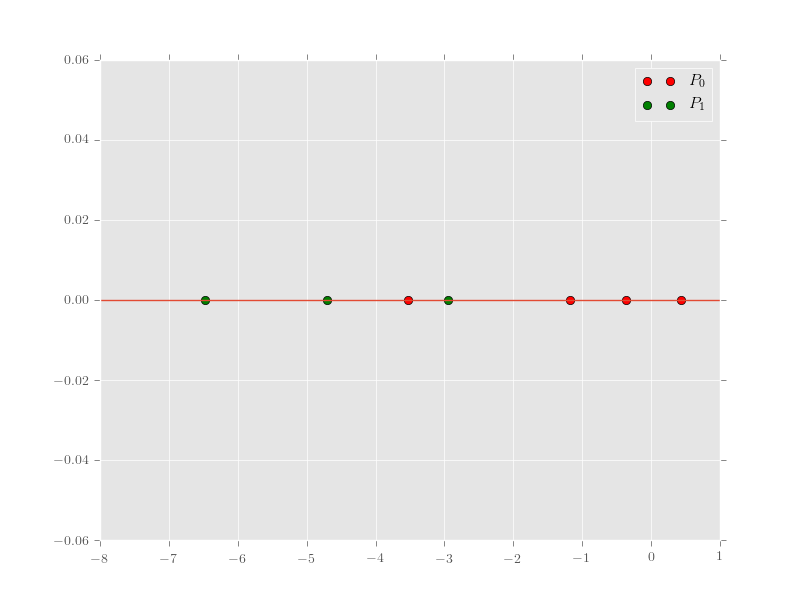
\includegraphics[width=0.9\textwidth]{aufg3.png}
	\caption{Projektion der Populationen auf Gerade}
\end{figure}

\section*{Aufgabe 4: \emph{Datenaufbereitung}}

\begin{itemize}

\item[a)]
\item[1.] Tokenizierung: Zerlegen eines Fließtextes in Tokens (kleine Einheiten) und anschließendes Löschen unbrauchbarer Tokens
\item[Bsp.:] Erstellung von Bbliotheken zu Natural Language Processing
\item[2.] Typ und Formatierung einzelner Einträge aneinander anpassen.
\item[Bsp.:] Gleiche Formatierung für Einträge von Daten oder Zeiten.
\item[3.] Ersetzen nicht eindeutiger Daten.
\item[Bsp.:] Lücken, NaNs, $\infty$ sinnvoll ersetzen oder löschen.
\item[4.] Ersetzen von missverständlichen Informationen.
\item[Bsp.:] Konstanten und fehlende Werte löschen.

\item[b)] Eine Normierung sorgt für eine bessere Vergleichbarkeit von Daten.
\item[c)] Löschen oder ersetzen von Daten.
\item[d)] Daten müssen miteinander kombiniert werden können. Zum Beispiel anpassen von Tabellenlängen beim Zusammenführen, gleiche Formatierung von Daten.
\end{itemize}